\documentclass{beamer}
\usetheme{STCE}
\usepackage{beamerfoils}
\uselanguage{German}
\languagepath{German}

\usepackage{epstopdf}

\usepackage{ucs} % Unicode - dependency of utf8x inputenc
\usepackage[utf8x]{inputenc} % "utf8x" uses "ucs"-package, better than "UTF8"
\usepackage[T1]{fontenc}
\usepackage{lmodern}

\usepackage[german]{babel}
\usepackage{amsmath, amssymb, amsxtra, amsthm, pxfonts}
\usepackage{epsfig,psfrag, epstopdf}
\usepackage{listings}

\usepackage{tikz}

\usepackage{nicefrac}


\beamertemplatenavigationsymbolsempty % turn off navigation bar

\lstloadlanguages{[ISO]C++, R}
\lstset{basicstyle=\small, numbers=left, numberstyle=\footnotesize, tabsize=2,  stepnumber=1, numbersep=5pt, breaklines=true, escapeinside={/*@}{@*/}}

\setbeamertemplate{footline}[frame number]

\MyLogo{
\centering

\includegraphics[width=0.12\textwidth]{./figures/logo.eps}
}

\begin{document}
\title{\centering

\includegraphics[width=0.25\textwidth]{./figures/logo.eps} \\ Numerische Bibliotheken}

\subtitle{Der $\chi^2$ und Kolmogorow-Smirnow Test}
\author{Christian Janßen (302530) \\ Fabian Ohler (280424) }
\date{6. August 2013}
\institute{
LuFG Informatik 12: Software and Tools for Computational Engineering}
\frame[plain]{\titlepage}

%%% Inhalt
\begin{frame}{Inhalt}
	\tableofcontents
\end{frame}

%%%Einführung
\section{Einführung}
\begin{frame}{\insertsection}
Themen dieses Vortrags:
	\begin{itemize}
		\item Statistik
			\begin{itemize}
			\item ist das Sammeln, Auswerten und Beurteilen von Daten
			\item dient als Bindeglied zwischen Daten und Hypothesen
			\end{itemize}		
		\item Numerische Bibliotheken
			\begin{itemize}
			\item stellen mathematische Algorithmen zur Verfügung wodurch eine eigene Implementation entfällt
			\item sind in diesem Vortrag NAG C und die Sprache R
			\end{itemize}
	\end{itemize}
\end{frame}

%%%Statistische Grundlagen
\section{Statistische Grundlagen}

\begin{frame}{\insertsection}
\begin{definition}
	\begin{description}[Punkt im Ergebnisraum]
	\item[Experiment] verschiedene mögliche Ausgänge
	\item[Ergebnisraum] Menge aller möglichen Ausgänge
	\item[Punkt im Ergebnisraum] ein konkreter Ausgang
	\item[Ereignis] Menge von Punkten im Ergebnisraum
	\item[P: Ergebnisraum $\rightarrow\mathbb{R}$] Wahrscheinlichkeitsfunktion
	\item[P(A)] Wahrscheinlichkeit für Ereignis A
	\end{description}
\end{definition}
\end{frame}

\begin{frame}{\insertsection}
\begin{example}[Münzwurf]
	\begin{description}[Punkt im Ergebnisraum]
	\item[Experiment] wirf eine (faire) Münze zwei Mal
	\item[Ergebnisraum] $E \coloneqq \{ZZ,ZK,KZ,KK\}$
	\item[Punkt im Ergebnisraum] z.\,B.~$KK \in E$
	\item[Ereignis] z.\,B.~mind.~1x Kopf: $\{ZK, KZ, KK\} \subseteq E$
	\item[P(A)] = $0.25 ~\forall A\in E$
	\item[P(mind.~1x Kopf)] = 0.75
	\end{description}
\end{example}
\end{frame}

\begin{frame}{\insertsection}
\begin{definition}
	\begin{description}[kumulierte Verteilungsfunktion]
	\item[Zufallsvariable X] \emph{sortiert} Punkte im Ergebnisraum
	\item[Dichtefunktion] $f(x) = P(X=x)$
	\item[kumulative Verteilungsfunktion] $F(x) = P(X \leq x)$
	\item[Quantil] $x_p: ~ P(X\leq x_p)\geq p$ und $P(X\geq x_p)\geq 1-p$
	\item[Median] $x_{0.5}$
	\item[Erwartungswert] $\mu = E(X) = \int x\cdot f(x) \text{d}x$
	\item[Varianz] $\sigma^2 = E[(X-\mu)^2]$
	\item[Standardabweichung] $\sigma = \sqrt{\sigma^2}$
	\end{description}
\end{definition}
\end{frame}

\begin{frame}{\insertsection}
\begin{block}{Normalverteilung $\mathcal{N}(\mu,\sigma^2)$}
	$\mu$ Erwartungswert, $\sigma^2$ Varianz \\
	kumulative Verteilungsfunktion:
	\begin{equation*}
	F(x) = \Phi\left(\frac{x - \mu}{\sigma}\right) = \frac{1}{\sqrt{2\pi\sigma}} \int_{-\infty}^{x}e^{-\frac{1}{2}[(y-\mu)/\sigma]^2}\textrm{d}y
	\end{equation*}
\end{block}
\end{frame}

\begin{frame}{\insertsection}
	\begin{figure}[htbp]
		\centering
		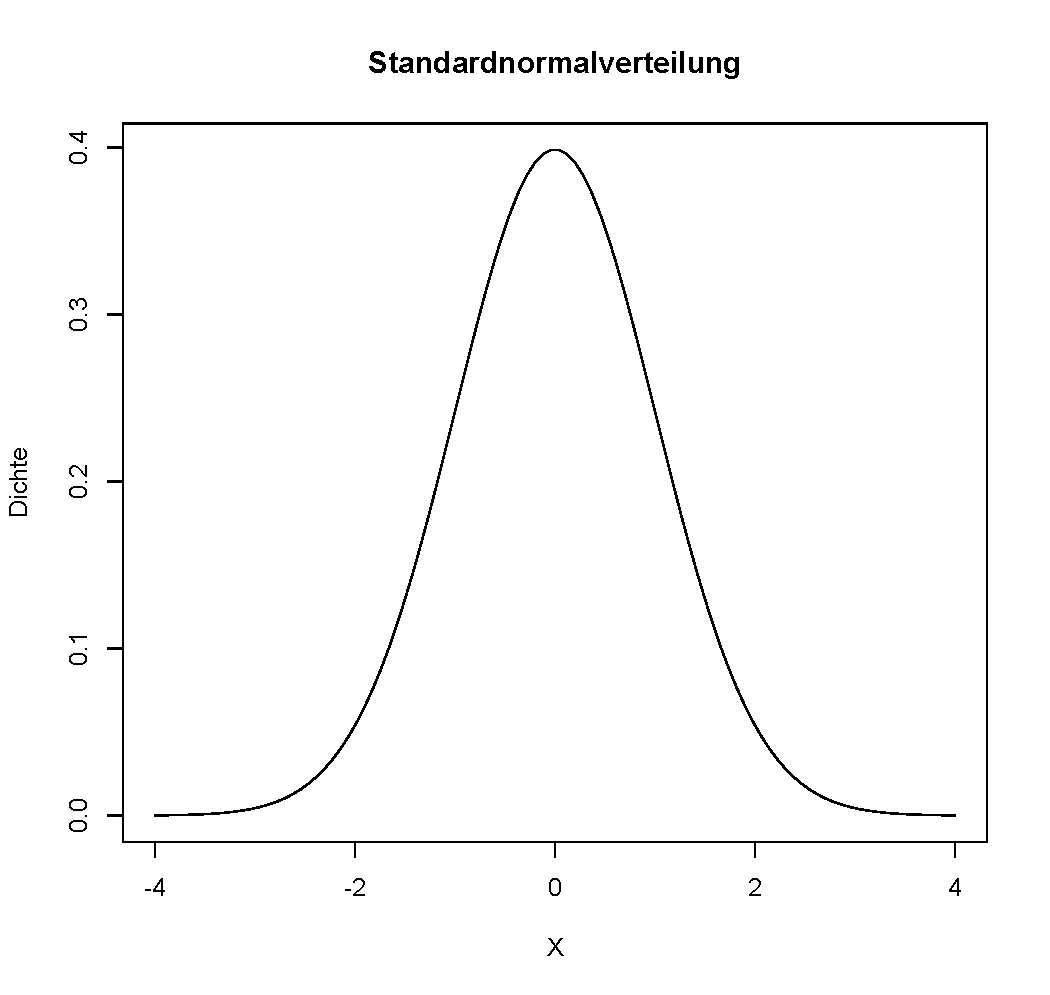
\includegraphics[height=0.99\textheight]{figures/standardnorm_empty}
	\end{figure}
\end{frame}
%quantil
\begin{frame}{\insertsection}
	\begin{figure}[htbp]
		\centering
		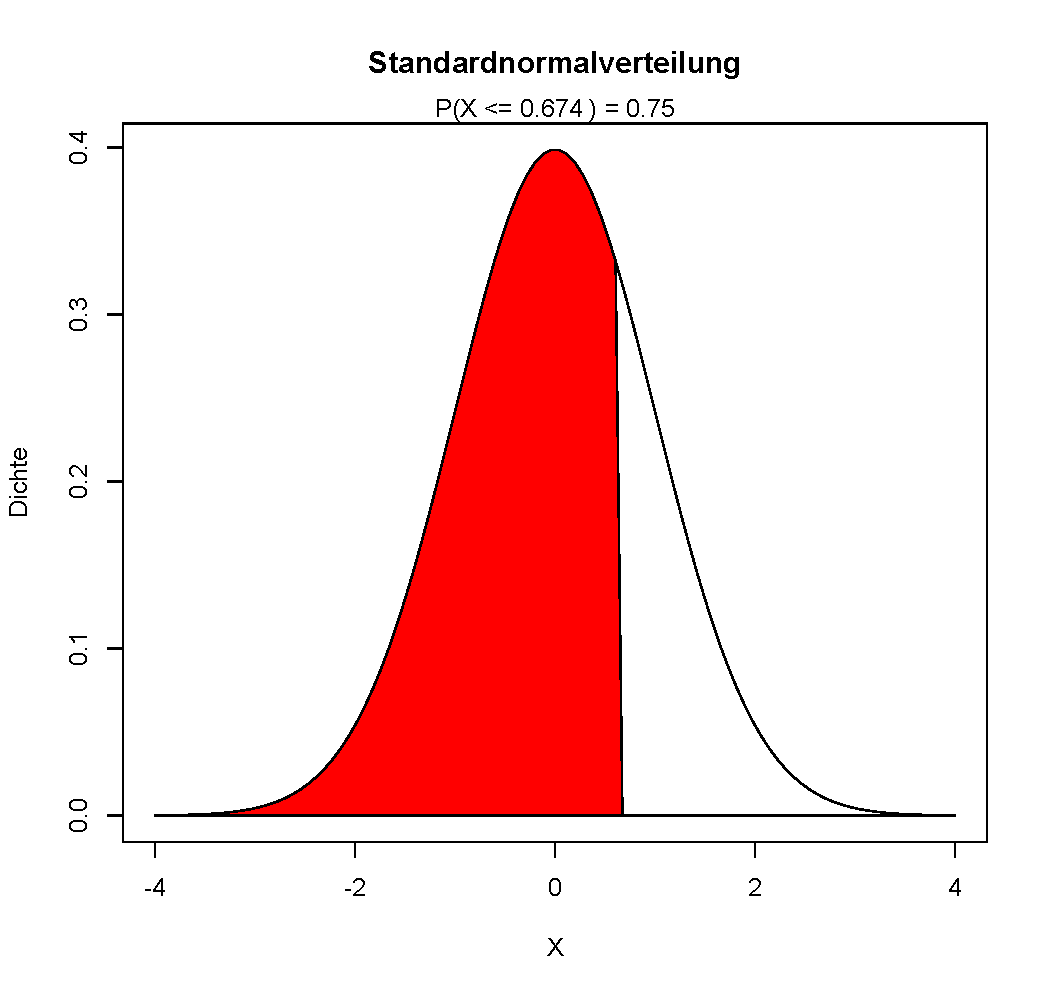
\includegraphics[height=0.99\textheight]{figures/standardnorm_quantil}
	\end{figure}
\end{frame}
%F
\begin{frame}{\insertsection}
	\begin{figure}[htbp]
		\centering
		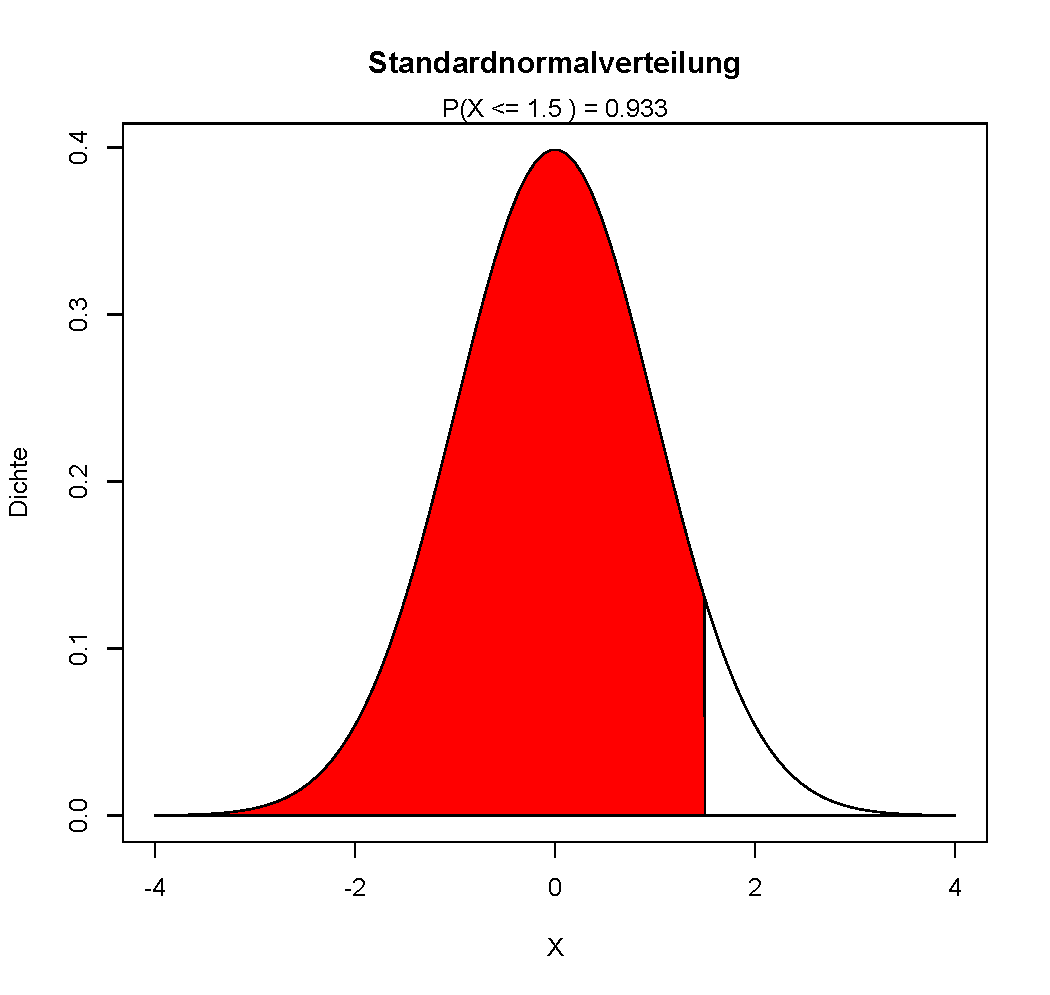
\includegraphics[height=0.99\textheight]{figures/standardnorm}
	\end{figure}
\end{frame}

\begin{frame}{\insertsection}
\begin{block}{Gleichverteilung $\mathcal{U}(a,b)$}
	$a$ Minimum, $b$ Maximum \\
	kumulative Verteilungsfunktion:
	\begin{equation*}
	F(x) = \left\{\begin{tabular}{ll}
	0 & for $x<a$ \\
	$\frac{x-b}{b-a}$ & for $a\leq x<b$ \\
	1 & for $x\geq b$ \\
	\end{tabular}\right.
	\end{equation*}
\end{block}
\end{frame}

\begin{frame}{\insertsection}
\begin{block}{Binomialverteilung $B(n,p)$}
	$n$ Anzahl der Erfolge, $p$ Wahrscheinlichkeit des Erfolgs bei booleschem Ergebnis \\
	kumulative Verteilungsfunktion:
	\begin{equation*}
	F(x) = \sum_{i\leq x} \genfrac(){0pt}{}{n}{i} p^{i}q^{n-i}
	\end{equation*}
\end{block}
\end{frame}


\begin{frame}{\insertsection}
\begin{block}{Chi-Quadrat-Verteilung $\chi^2(k)$}
	$k$ Anzahl der Freiheitsgrade \\
	kumulative Verteilungsfunktion:
	\begin{equation*}
	F(x) = \left\{\begin{tabular}{ll}
	$\int_{0}^{x} \frac{y^{(k/2)-1}e^{(y/2)}}{2^{k/2}\Gamma(k/2)}\textrm{d}y$ & if $x>0$ \\
	0 & if $x\leq 0$
	\end{tabular}\right.
	\end{equation*}
\end{block}
\begin{example}
	$X_1, \ldots X_k$ unabhängig \& gleich normalverteilt \\
	$Y = \sum_{i=1}^{k}X_i^2$ ist $\chi^2$-verteilt mit $k$ Freiheitsgraden
\end{example}
\end{frame}

\begin{frame}{\insertsection}
\begin{definition}
	\begin{description}[Zufallsstichprobe]
	\item[Grundgesamtheit] alle relevanten Elemente
	\item[Stichprobe] Teilmenge der Grundgesamtheit
	\item[Zufallsstichprobe] Stichprobe, bei der jedes Element gleich wahrscheinlich war
	\item[] 
	\end{description}
\end{definition}
\begin{definition}[empirische Verteilungsfunktion]
	Zufallsstichprobe, Größe $n$
	\begin{equation*}
	S(x) = \frac{1}{n}(\text{\#Stichprobenelemente}\leq x)
	\end{equation*}
\end{definition}
\end{frame}

\begin{frame}{\insertsection}
\begin{definition}[Qualität eines Schätzers]
	\begin{description}[Zuverlässigkeit]
	\item[Präzision] Nähe zum echten Wert
	\item[Zuverlässigkeit] Wahrscheinlichkeit, korrekt zu sein
	\end{description}
\end{definition}
\begin{example}[Punktschätzer, hohe Präzision, geringe Zuverlässigkeit]
	\begin{description}[Beispiele]
	\item[Beispiele] Mittelwert, Stichprobenvarianz Punktschätzer für Erwartungswert, Varianz
	\end{description}
\end{example}
\begin{example}[Konfidenzintervall, niedere Präzision, hohe Zuverlässigkeit]
	\begin{description}[Beispiel]
	\item[Beispiel] \glqq Wir sind zu 90\% sicher, dass weniger als 1\% unserer Produkte fehlerhaft sind\grqq.
	\end{description}
\end{example}
\end{frame}

\begin{frame}{\insertsection}
\begin{block}{statistisches Schließen}
	Stichprobe $\Rightarrow$ Grundgesamtheit (Induktion)
	\\
	Gegenteil: Deduktion
\end{block}
\begin{block}{Hypothesen-Tests}
	Methode der Entscheidungsfindung:\\
	\emph{Kann allg.~Aussage über Grundgesamtheit wegen Stichprobe angenommen werden?}
\end{block}
\begin{definition}[Hypothese (lt.~Wiktionary)]
	unbewiesene (wissenschaftliche) Annahme, die noch eines Beweises bedarf
\end{definition}
\end{frame}

%%%Kolmogorow-Smirnow Test
\section{Kolmogorow-Smirnow Test}
\begin{frame}{\insertsection}
Kolmogorow-Smirnow Test hat zwei Anwendungen:\\
	\begin{itemize}
		\item[1.] Pr\"uft Mengen $X$ und $ Y$ auf gleiche Wahrscheinlichkeitsverteilung \\
		\item[2.] Pr\"uft Menge $X$ auf spezifizierte Wahrscheinlichkeitsverteilung $F(x)$ \\
			\[S(x)=F(x)\]
			\begin{center}$\rightarrow$ Anpassungsg\"utetest\end{center}
	\end{itemize}
\end{frame}

	%%%Mathematischer Hintergrund
\subsection{Mathematischer Hintergrund}

\begin{frame}{\insertsubsection}
Anwendung des Anpassungsg\"utetests:
	\begin{itemize}
		\item Menge $X$ aufsteigend sortieren, $x_1\le ...\le x_n$
		\item<2-> Bilden der empirischen Verteilungsfunktion $S(x)$	
		\only<2>{ $$S(x)=\frac{1}{n}\sum^{n}_{i=1}I_{x_i\le x}$$}
		\item<3-> Spezifizieren der angenommenen Verteilungsfunktion $F(x)$
		\item<3-> Aufstellen der Nullhypothese $H_0$ und der Alternativhypothese $H_1$
		\only<3>{$$H_0:S(x)=F(x)$$ $$H_1:S(x)\neq F(x)$$}
		\item<4-> Ermitteln der Teststatistik $D_n$
		\only<4>{ $$D_n=\max(d_0,d_1)$$ $$ d_0=\max_x|S(x)-F(x)|,$$ $$d_1=\max_x|S(x_{i-1})-F(x_i)|$$ }
		\item<5->Wenn $D_n>D_\alpha$ wird die Nullhypothese verworfen
	\end{itemize}
\end{frame}

	%%%Beispiel

\begin{frame}{\insertsubsection}
Ein Beispiel:\\
	\begin{itemize}
		\item Beobachtungen:
			\begin{table}[h]
			\center
			\begin{tabular}{c|c|c|c|c|c|c|c|c|c}
			$x_1$	&$x_2$	&$x_3$	&$x_4$	&$x_5$	&$x_6$	&$x_7$	&$x_8$	&$x_9$	&$x_{10}$\\
			\hline
			1	&1.1	&1.2	&1.6	&1.7	&2.1	&2.1	&2.4	&2.4	&2.5	\\
			\end{tabular}
			\begin{tabular}{c|c|c|c|c|c|c|c|c|c}
			$x_{11}$	&$x_{12}$	&$x_{13}$	&$x_{14}$	&$x_{15}$	&$x_{16}$	&$x_{17}$	&$x_{18}$	&$x_{19}$	&$x_{20}$\\
			\hline
			2.6	&2.6	&2.6	&2.7	&2.8	&3	&3.3	&3.5	&3.8	&4.2\\
			\end{tabular}
			\end{table}
		\item Hypothesen: $$H_{Franz}:S(x)=\Phi(x|3.5;1)$$ $$H_{Paul}:S(x)=\Phi(x|3;0.7)$$
	\end{itemize}
\end{frame}

\begin{frame}{\insertsubsection}
Berechnung der Werte:\\
	\begin{itemize}
		\item Werte der Verteilungsfunktionen
			\begin{table}[ht]
			\center
			\begin{tabular}{c|c|c|c|c}
			$i$ 	& $x_i$ 	& $S(x_i)$ 	& $\Phi (x_i|3;0,7)$ 	& $\Phi (x_i|3,5;1)$ 	\\
			\hline
			1	&	1	&	0.05	&	0.002137	&	0.006210	\\
			12	&	2.6	&	0.65	&	0.283855	&	0.184060	\\
			15	&	2.8	&	0.75	&	0.387548	&	0.241964	\\
			20	&	4.2	&	1	&	0.956762	&	0.758036	\\
			\end{tabular}
			\end{table}
		\item Werte der Teststatistik
			\begin{table}[ht]
			\center
			\begin{tabular}{c|c|c|c|c}
			$i$ 	& $d_{0,Paul}(x_i)$ 	& $d_{1,Paul}(x_i)$ 	& $d_{0,Franz}(x_i)$ 	& $d_{1,Franz}(x_i)$ 	\\
			\hline
			1	&	0.047863	&	0.002137	&	0.043790	&	0.006210	\\
			12	&	0.366145	&	0.366145	&	0.465940	&	0.465940	\\
			15	&	0.362452	&	0.312452	&	0.508036	&	0.458036	\\
			20	&	0.043238	&	0.006762	&	0.241964	&	0.191964	\\
			\end{tabular}
			\end{table}
	\end{itemize}
\end{frame}

\begin{frame}{\insertsubsection}
Auswertung der Teststatistiken:\\
	\begin{itemize}
		\item $D_{n,Franz}=0.508036$ und $D_{n,Paul}=0.366145$
		\item $D_\alpha=0.294$
	\end{itemize}
Somit sind beide Hypothesen verworfen.
\end{frame}

	%%%NAG C
\subsection{Implementierung in NAG C}
\begin{frame}[fragile]{\insertsubsection}
In NAG C: \lstinline[language=C++]$g08cbc$ oder \lstinline[language=C++]$nag_1_sample_ks_test$ mit folgenden Parametern:\\
\begin{center}\lstinline[language=C++]$g08cbc(n, x[], dist, par[], estima, dtype, *d, *z, *p, *fail)$\end{center}
Die Eingabeparameter sind die Folgenden:
	\begin{description}
		\item[n] -- Integer der die Anzahl der Beobachtungen speichert
		\item[x{[n]}] -- Double Array mit den Beobachtungen $x_1...x_n$
		\item[dist] -- Nag\_Distribution spezifiziert $F(x)$
		\item[par{[2]}] -- Enthält optional weitere Parameter für $dist$
		\item[estima] -- Nag\_ParaSupplied falls $par$ gegeben ist oder Nag\_ParaEstimated wenn die Parameter von NAG bestimmt werden sollen
		\item[dtype] -- definiert Nag\_TestStatistics
	\end{description}
\end{frame}

\begin{frame}[fragile]{\insertsubsection}
$dtype$ muss einer der drei folgenden Werte zugewiesen werden:
	\begin{itemize}
		\item Nag\_TestStatisticsDAbs
		\item Nag\_TestStatisticsDPos
		\item Nag\_TestStatisticsDNeg
	\end{itemize}
	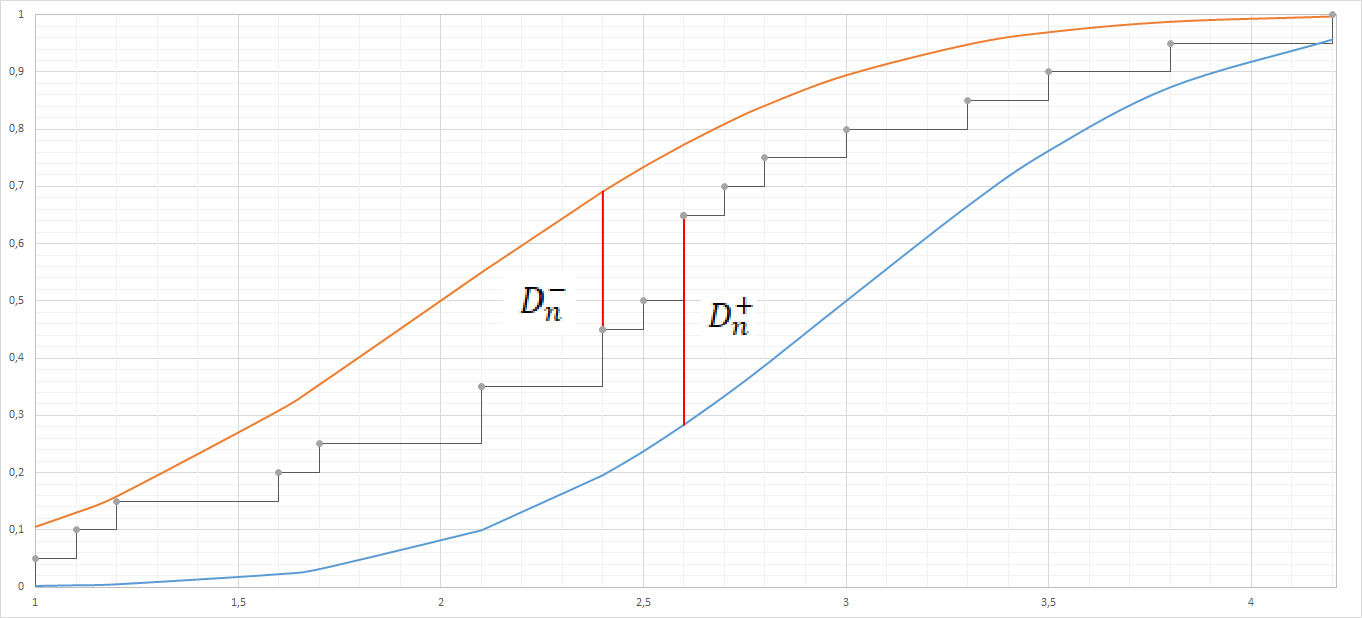
\includegraphics[width=1.0\textwidth]{figures/diagramKSd-d+.png}
\end{frame}

\begin{frame}[fragile]{\insertsubsection}
\begin{center}\lstinline[language=C++]$g08cbc(n, x[], dist, par[], estima, dtype, *d, *z, *p, *fail)$\end{center}
Folgende Werte werden von der Funktion beschrieben:
	\begin{description}
		\item[*d] -- Double mit dem Wert der Teststatistik
		\item[*z] -- Double mit dem $z$ Wert
		\item[*p] -- Double mit $p$ Wert
		\item[*fail] -- NagError mit etwaigen Fehlerbeschreibungen
	\end{description}
\end{frame}

	%%%R
\subsection{Alternative Bibliotheken}
\begin{frame}{\insertsubsection}
R als alternative Bibliothek mit der folgenden Methode: 
\begin{center}\lstinline[language=R] $ks.test(x, y, ..., alternative)$\end{center}
\begin{description}
\item[x] -- Numerischer Vektor mit  allen Beobachtungen
\item[y] -- String welche die Nullverteilung beschreibt
\item[...]-- Strings mit Parametern für $y$
\item[alternative]-- definiert welche Teststatistik berechnet wird
\end{description}
R generiert folgende Rückgabe:
\begin{description}
\item[statistic] -- Teststatistik welche in $alternative$ festgelegt wurde
\item[p.value] -- p Wert
\item[alternative] -- gewählter Wert für $alternative$
\item[method] -- genutzter Test
\item[data.name] -- Namen der Daten
\end{description}

\end{frame}



%%%$\chi^2$ Test
\section{$\chi^2$ Test}
\subsection{Mathematischer Hintergrund}
\subsection{Implementierung in NAG C}
\subsection{Alternative Bibliotheken}
\begin{frame}
\frametitle{$\chi^2$ Test}
\end{frame}

%%%Live Demo
\section{Live Demo}

\begin{frame}{\insertsection}
\center
\Huge Live Demo
\end{frame}

%%%Zusammenfassung
\section{Vergleich}

\begin{frame}{\insertsection}

\begin{columns}
\begin{column}{.48\textwidth}
R:
	\begin{itemize}
		\item freie Verfügbar
		\item leicht handhabbar
	\end{itemize}
\vspace{1cm}
NAG C:
	\begin{itemize}
		\item kostenpflichtig
		\item komplex
		\item Support
	\end{itemize}
\end{column}

\hfill
\begin{column}{.48\textwidth}
KS-Test:
	\begin{itemize}
		\item erstellen der empirischen Verteilungsfunktion
		\item benötigt weniger Beobachtungen als $\chi^2$
	\end{itemize}
\vspace{1cm}
$\chi^2$-Test:
	\begin{itemize}
		\item erstellen von Klassen
	\end{itemize}
\end{column}
\end{columns}




\end{frame}


\end{document}
